%
% REVISION 2 - added supplementary information figure.
%
%%%%%%%%%%%%%%%%%%%%%%%%%%%%%%%%%%%%%%%%%%%%%%%%%%%%%%%%%%%%%%%%%%%%%
%% This is a (brief) model paper using the achemso class
%% The document class accepts keyval options, which should include
%% the target journal and optionally the manuscript type. 
%%%%%%%%%%%%%%%%%%%%%%%%%%%%%%%%%%%%%%%%%%%%%%%%%%%%%%%%%%%%%%%%%%%%%
\documentclass[journal=acsodf,manuscript=article]{achemso}

%%%%%%%%%%%%%%%%%%%%%%%%%%%%%%%%%%%%%%%%%%%%%%%%%%%%%%%%%%%%%%%%%%%%%
%% Place any additional packages needed here.  Only include packages
%% which are essential, to avoid problems later. Do NOT use any
%% packages which require e-TeX (for example etoolbox): the e-TeX
%% extensions are not currently available on the ACS conversion
%% servers.
%%%%%%%%%%%%%%%%%%%%%%%%%%%%%%%%%%%%%%%%%%%%%%%%%%%%%%%%%%%%%%%%%%%%%
\usepackage[version=3]{mhchem} % Formula subscripts using \ce{}
\usepackage{gensymb} %used for degree symbol, use as \degree

%%%%%%%%%%%%%%%%%%%%%%%%%%%%%%%%%%%%%%%%%%%%%%%%%%%%%%%%%%%%%%%%%%%%%
%% If issues arise when submitting your manuscript, you may want to
%% un-comment the next line.  This provides information on the
%% version of every file you have used.
%%%%%%%%%%%%%%%%%%%%%%%%%%%%%%%%%%%%%%%%%%%%%%%%%%%%%%%%%%%%%%%%%%%%%
%%\listfiles

%%%%%%%%%%%%%%%%%%%%%%%%%%%%%%%%%%%%%%%%%%%%%%%%%%%%%%%%%%%%%%%%%%%%%
%% Place any additional macros here.  Please use \newcommand* where
%% possible, and avoid layout-changing macros (which are not used
%% when typesetting).
%%%%%%%%%%%%%%%%%%%%%%%%%%%%%%%%%%%%%%%%%%%%%%%%%%%%%%%%%%%%%%%%%%%%%
%\newcommand*\mycommand[1]{\texttt{\emph{#1}}} 

%\usepackage{lineno}
%\linenumbers

%%%%%%%%%%%%%%%%%%%%%%%%%%%%%%%%%%%%%%%%%%%%%%%%%%%%%%%%%%%%%%%%%%%%%
%% Meta-data block
%% ---------------
%% Each author should be given as a separate \author command.
%%
%% Corresponding authors should have an e-mail given after the author
%% name as an \email command. Phone and fax numbers can be given
%% using \phone and \fax, respectively; this information is optional.
%%
%% The affiliation of authors is given after the authors; each
%% \affiliation command applies to all preceding authors not already
%% assigned an affiliation.
%%
%% The affiliation takes an option argument for the short name.  This
%% will typically be something like "University of Somewhere".
%%
%% The \altaffiliation macro should be used for new address, etc.
%% On the other hand, \alsoaffiliation is used on a per author basis
%% when authors are associated with multiple institutions.
%%%%%%%%%%%%%%%%%%%%%%%%%%%%%%%%%%%%%%%%%%%%%%%%%%%%%%%%%%%%%%%%%%%%%

\author{Aaron J. Celestian}
\email{acelesti@nhm.org}
\affiliation{Department of Mineral Sciences, Natural History Museum of Los Angeles County}

\author{Jason Lively}
\affiliation{Department of Geography and Geology, Western Kentucky University}

\author{Wenqian Xu}
\affiliation{X-ray Science Division, Advanced Photon Source, Argonne National Laboratory, Argonne, IL 60439}


%%%%%%%%%%%%%%%%%%%%%%%%%%%%%%%%%%%%%%%%%%%%%%%%%%%%%%%%%%%%%%%%%%%%%
%% The document title should be given as usual. Some journals require
%% a running title from the author: this should be supplied as an
%% optional argument to \title.
%%%%%%%%%%%%%%%%%%%%%%%%%%%%%%%%%%%%%%%%%%%%%%%%%%%%%%%%%%%%%%%%%%%%%
\title[Cs and H Exchange into Gaidonnayite]
{\textit{In Situ} Cs and H Exchange into Gaidonnayite and Proposed Mechanisms of Ion Diffusion}

%%%%%%%%%%%%%%%%%%%%%%%%%%%%%%%%%%%%%%%%%%%%%%%%%%%%%%%%%%%%%%%%%%%%%
%% Some journals require a list of abbreviations or keywords to be
%% supplied. These should be set up here, and will be printed after
%% the title and author information, if needed.
%%%%%%%%%%%%%%%%%%%%%%%%%%%%%%%%%%%%%%%%%%%%%%%%%%%%%%%%%%%%%%%%%%%%%

\keywords{zeolite, microporous, remediation, ion exchange}

%%%%%%%%%%%%%%%%%%%%%%%%%%%%%%%%%%%%%%%%%%%%%%%%%%%%%%%%%%%%%%%%%%%%%
%% The manuscript does not need to include \maketitle, which is
%% executed automatically.
%%%%%%%%%%%%%%%%%%%%%%%%%%%%%%%%%%%%%%%%%%%%%%%%%%%%%%%%%%%%%%%%%%%%%
\begin{document}

%%%%%%%%%%%%%%%%%%%%%%%%%%%%%%%%%%%%%%%%%%%%%%%%%%%%%%%%%%%%%%%%%%%%%
%% The "tocentry" environment can be used to create an entry for the
%% graphical table of contents. It is given here as some journals
%% require that it is printed as part of the abstract page. It will
%% be automatically moved as appropriate.
%%%%%%%%%%%%%%%%%%%%%%%%%%%%%%%%%%%%%%%%%%%%%%%%%%%%%%%%%%%%%%%%%%%%%
\begin{tocentry}
\emph{In situ} Cs and H ion exchange was performed to monitor the
dynamics of cation size exchange at ambient and elevated temperature in
gaidonnayite. At elevated temperature, the rate and capacity of Cs
exchange into Na-gaidonnayite increased over the comparable~experiment
at ambient temperatures. This study demonstrated the effect of host
cation size and temperature on the Cs exchange into this microporous
mineral.
\\ \\ \\ \\ \\ \\ \\ \\ \\ 
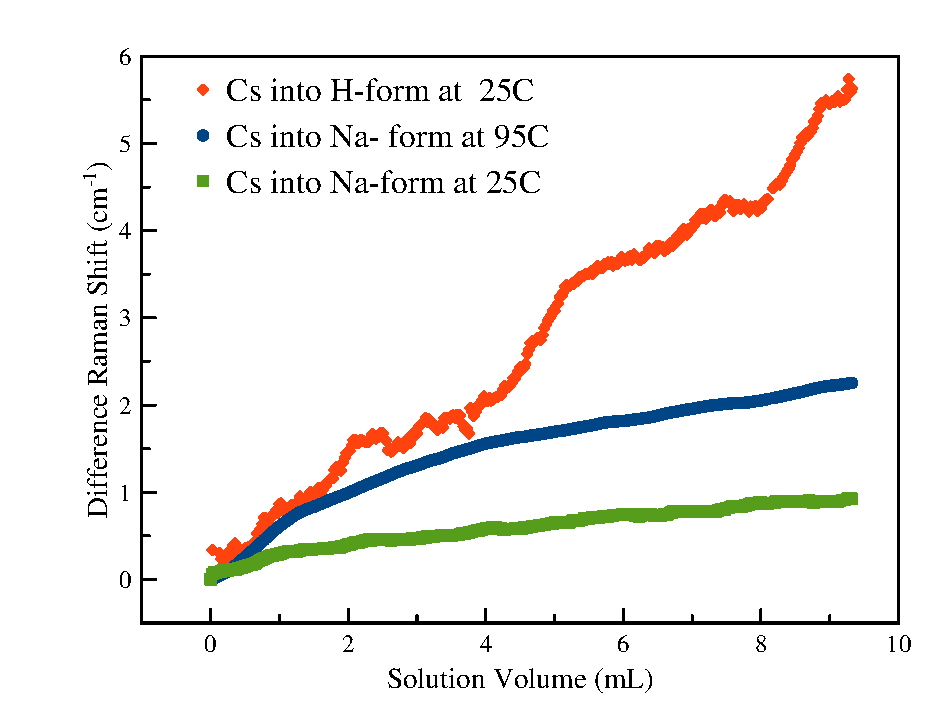
\includegraphics[width=8.25cm]{figures/For-Table-of-Contents-Only.pdf}
\captionof*{figure}{For Table of Contents Only}
\end{tocentry}



\begin{abstract}
The microporous mineral gaidonnayite \ce{Na_{2}ZrSi_{3}O_{9} . 2H_{2}O} was studied to better understand its ion exchange mechanisms, specifically for \ce{Cs+} and \ce{H+} ions. \textit{In situ} Raman spectroscopy, \textit{in situ} X-ray diffraction (XRD), simultaneous thermogravimetric analysis and differential scanning calorimetry (TGA/DSC), and \textit{in situ} X-ray fluorescence were used to determine the exchange processes involved. The Raman spectra contain strong peaks that can be attributed to the vibrational modes for the 3MR symmetric stretch at $\mathrm{500 \ cm^{-1}}$ Si-O-Zr-O chain stretches at $\mathrm{938 \ cm^{-1}}$, and \ce{Si-O} stretching in the $\mathrm{1000-1100 \ cm^{-1}}$ range. The most prominent Raman shift during ion exchange is found near the $\mathrm{520 \ cm^{-1}}$ peak, which corresponds to distortions of the 3MR substructure of gaidonnayite. In all instances of this study, the 3MR exhibited the highest amount of distortion during ion exchange, and the evolution of this distortion is compared to unit-cell changes as measured from XRD data and elemental changes via XRF. The correlations between the Raman, XRD, and XRF data show rapid deformation of the 3MR during the onset of \ce{H+} ion exchange in the Na form of gaidonnayite. Even when unit-cell volume changes were small ($<3$ \AA$^3$) as in the cases for \ce{Cs+} into Na-gaidonnayite and \ce{Cs+} into H-gaidonnayite, significant changes in $\mathrm{\approx 520 \ cm^{-1}}$  peak were measured. By comparing XRD data, Raman data, and verifying the cation uptake by XRF, we were able to identify and confirm conformational changes and distortions in the crystal structure before, during, and after \ce{Cs+} and \ce{H+} exchange. Cs exchange occurred the fastest and with the greatest capacity when starting in the H-form at room temperature, and at elevated temperatures when starting in the Na-form.
\end{abstract}


\section{Introduction}  \label{sec_introduction}

Ion exchange and selectivity within microporous materials have been widely used in both industrial and environmental applications. Much effort has been made to synthesize microporous materials that improve upon the ion sieving properties of their natural counterparts and to increase ion selectivity. Microporous materials contain tunnel-like pores (up to 2 nm) throughout their crystalline framework. The pores are commonly occupied by \ce{H2O} molecules and cations to charge balance the negative charge on the framework. Incorporation of \ce{H+} into the structure of these materials enhances catalytic cracking of hydrocarbons \cite{Mortensen_2011,Huber_2007,Guisnet_1992,Kramer_1993,Narbeshuber_1995,Kissin_2001}. Microporous materials, specifically zirconium and titanium silicates, have been used in gas separation  \cite{Kuznicki_2001,Marathe_2005,Delgado_2008,Mani_2015,Navascu_s_2006}. Environmental applications include purification of groundwater \cite{Bortun1997}, remediation of agricultural impacts \cite{Mumpton_1999}, and removal of heavy metals generated through mining \cite{motsi2009adsorption}, in nuclear reactors \cite{Mishra2006}, and biowastes \cite{simon2015recovery}. Gaidonnayite is a zirconium silicate microporous material that is easily synthesized and has a wide range of thermal stability, both of which are advantageous for selective ion sequestration applications. However, gaidonnayite has generally not been considered a viable sequestration material previously because of its rarity (only known in abundance from a few localities worldwide, e.g. Mt. St. Hilaire, see mindat.org), and its relatively small channel diameter, though we demonstrate in this study that those properties are not limiting factors.

Cesium-137 is a major gamma radiation emitter in spent nuclear fuel that poses threats to the environment \cite{Galadima2015,Wilmarth2011,Mishra2006,Bortun1997} and health \cite{Redman1972,Ramalho1991,Pinsky1981}. Therefore, it would be advantageous to find radiation- and geologically-stable materials that can selectively absorb cesium, thereby preventing this toxin from becoming biologically accessible \cite{M_ller_2002,Tripathi_2003,Ewing_2004,Hughes_2015,Misaelides2011,Borai_2009,Ewing_2001,Shi_2006}.  


Materials that have been used for ion exchange of \ce{Cs+} from aqueous environments include glasses (e.g. \cite{Mastelaro2018,Peterson2018,Tollefson2017,Yang2017}), clay minerals (e.g. \cite{Dobre2018,Fernandes2016,Jolin2016,Pusch_1992,Y_ld_z_2011,Zhang_2017}), microporous materials (e.g.  \cite{Celestian_2013,Celestian_2005,Fewox2011,Borai_2009,WoldeGabriel_1993,Marinin_2000,Dyer_1984}), and other materials and methods (e.g. \cite{van_Deventer_2007,Romanchuk_2013,Misaelides_2011,Manos_2008,Entry_1999,Mertz_2013,Riley_2013}). One concern with microporous materials is their relatively low thermal stability, a potential problem with high-temperature interactions in nuclear reactors and around un-cooled spent nuclear fuel pellets \cite{Ewing_2015,Weber_1997}. The molecular \ce{H2O} typically dehydrates out of zeolitic structures around 400 \degree C, often leading to instability. However, this study demonstrates that ion exchange in gaidonnayite may be enhanced at elevated temperatures below the dehydration temperatures of \textit{ca.} 300 \degree C, suggesting that the optimal temperature ranges for other microporous ion exchangers may be higher than expected.

Previous time-resolved ion exchange work on zeolites and microporous materials  (e.g. \cite{Norby_1996,Norby_1998,Dalconi_2003,Celestian_2010}) yielded valuable information on ion exchange dynamics. Static experimental studies are ideal for creating structural, molecular, and thermodynamic models, but structural transitions (and therefore the pathways of ion diffusion) between end-members are not captured in those studies. \textit{In situ} and \textit{in operando} studies obtain data while the material is undergoing change in varying environmental conditions, and therefore the mechanisms of the exchange processes can be better modeled. Certain compromises have to be made in order to collect data that will capture chemical processes in near real-time. The most significant compromise is the fast data collection times that span $\approx$ 30 seconds for X-ray diffraction (XRD) and Raman spectroscopy data (e.g. \cite{Celestian_2010}), and longer for X-ray fluorescence (XRF) data (60 seconds, or more; this study). These data collection times are dependent on the material being analyzed and instrumentation being used (e.g. synchrotron vs. seal-tube X-ray source).

Even with these compromises, \textit{in situ} studies can reveal transient structural changes and subtle conformation changes in the crystal structure, as demonstrated in studies of \ce{Cs+}, where short-range titania polyhedral distortions were observed prior to long-range (space group and unit-cell) crystallographic changes. However, \textit{in situ} studies need good starting parameters (e.g. crystallographic models, chemical constraints, etc.) to help constrain crystal structure model refinements and aid in the interpretation of Raman spectroscopy and XRD data. By combining the results of separate, but identical, experiments of cation exchange into gaidonnayite using Raman spectroscopy, XRD, and XRF we aim to gain a better understanding between short-range molecular distortions prior to long-range crystallographic changes in the mineral. In the current study, we are investigating the use of gaidonnayite, which is a microporous zeolitic mineral, for its ion exchange mechanisms for both \ce{H+} and \ce{Cs+} cations. The results of this work are intended to inform future models of \ce{Cs+} and \ce{H+} ion exchange processes for application in industrial and environmental sciences.

\subsection{Crystal Structure of Gaidonnayite and Hypothetical Ion Exchanged Forms}

\label{xtl_structures_hypothetical_exchange}  %xtl_structures_hypothetical_exchange

Gaidonnayite is an orthorhombic (P2\textsubscript{1}nb, \ce{Na_2ZrSi_3O_9 . 2H_2O}) microporous single chain silicate with minor ring
structures \cite{Chao1985}. The ring structures are comprised of a
series of 7MRs and 3MRs (see Figure {\ref{fig_gaid_7mr3mr}}),
built from both zirconia and silica polyhedra.   The size of the 7MR
pore space shown in Figure {\ref{fig_gaid_7mr3mr}} can be
changed by altering the bend angles in the 3MR, and this 3MR dihedral
angle changes with changing host cation.



\begin{figure}[h!] %fig_gaid_7mr3mr  
\begin{center}
\includegraphics[width=1.00\columnwidth]{figures/gaidonnayite_7MR_3MR.png}
\caption{{Polyhedral crystal structure showing the 7MR and 3MR substructures of the gaidonnayite framework.  \ce{ZrO_6} octohedra are green, \ce{SiO_4} tetrahedra are blue. Extra-framework cations removed for clarity.
{\label{fig_gaid_7mr3mr}}%
}}
\end{center}
\end{figure}


Theoretical calculations using energy-minimization implemented in
CrystalMaker (v9.2) were used to calculate optimized positions of Cs1
and Cs2 (corresponding to the Na1 and Na2 sites) in the gaidonnayite structure.  Because the computations are intensive, each cluster around Cs1 and Cs2 was calculated separately using a 16 \AA\ diameter cluster around the cation of interest that included at least 3\textsuperscript{rd} nearest neighbor sites.  Atomic sites in the center of the cluster were taken into account for the final
analysis, while atomic sites on the edges of the cluster were ignored
because of bond relaxation effects.  \ce{H} sites were not modeled as there
were many possible framework \ce{OH-} sites, and
\ce{H2O} would also need to be modeled (not done in this
computational analysis or in this study) for long-range structural stabilization of the H-bond network commonly found in microporous materials.  After placing
a \ce{Cs+} cation at the location of the Na2 and Na1 sites separately,
we allowed the models to relax and observed the movement of the
\ce{Cs+} atoms in the structure.  At the end of the first set of calculations, we found that Cs2 is centered in the large cage (Figure {\ref{fig_cage_view}}) with calculated Cs-O bond distances between 3.0 \AA\ and 3.4 \AA. At the end of the second set of calculations, the position of Cs1 (directly
exchanged for the Na1 site) is located in a smaller cage and maintained
chemically unreasonable bond-lengths, with several Cs-O bonds less than 2.8 \AA\ after energy minimization, and therefore it was determined that the Na1 site
is not likely to be a stable exchange site for \ce{Cs+}.  
Solvent-accessible void space was also calculated to visualize channel
geometry and connectivity.  The large cages are connected by 7MR
windows, which form a corrugated 1-dimensional channel
(Figure {\ref{fig_channel_view}}) that hosts the hydrated Na2
site near the center of its 7MR window.  


\begin{figure}  %fig_cage_view      
\begin{center}
\includegraphics[width=0.70\columnwidth]{figures/gaidonnayite_cages2_copy_2.png}
\caption{{The cage structure (cyan polyhedron) found in gaidonnayite is located at
the intersection of the 7MRs, with adjoining 3MR shown. The theoretical
Cs2 position in the center of the cage has an average bond length of 3.2
\AA\ (typical of Cs)\cite{Batsanov_2001}. Na2 position (yellow) shown is
located 1.3 \AA\ closer to the cage. The O sites are shown in red. The
irregular cage is centered at  $1/x \approx 0.507$, $1/y \approx 0.652$,
$1/z \approx 0.847$. Maximum and minimum cage diameters are
9.3 \AA\ and 6.2 \AA, respectively.
{\label{fig_cage_view}}%
}}
\end{center}
\end{figure}


\begin{figure}[h!] %fig_channel_view    
\begin{center}
\includegraphics[width=0.70\columnwidth]{figures/gaidonnayite_CHANNELS_anotated.jpg} 
\caption{{Cross-section of gaidonnayite channel interior is shown as darker
colors, the exterior of the channels are shown as lighter tan. Open
space is occupied by framework atoms, but are omitted for clarity. 
Larger cavities are the cages and smaller 7MR channels (labeled on figure).  Red vector is
{[}100{]}, green vector is {[}010{]}, and blue vector is {[}001{]} axial
directions.  Void space calculations performed in
OLEX2 \cite{Dolomanov_2009}.
{\label{fig_channel_view}}%
}}
\end{center}
\end{figure}

\section{Methods}

{\label{methods_section}}  %methods_section

\subsection{Gaidonnayite Materials}

{\label{methods_gaid_materials}}  %gaid_materials_methods

The materials used for \emph{in situ} analyses of gaidonnayite were
natural and synthetic samples.  Natural samples were obtained from the
Natural History Museum of Los Angeles catalog numbers 68497 through
68500, Poudrette quarry, Mount St. Hilaire, Quebec, Canada.  The
Na-gaidonnayite form was synthesized using previously published
methods \cite{Lin_1999}. The crystals were filtered and rinsed with
deionized \ce{H2O} and set aside to air dry at ambient
temperature. The crystals were verified to be gaidonnayite by both Raman
and XRD.  The resulting crystals were less than 10 microns in size and
unsuitable for single-crystal diffraction experiments. The rarity of
large natural gaidonnayite crystals prevented their use for
\emph{in-situ} experiments because not enough material can be obtained.  Attempts were made to use natural crystals of a suitable size for
single-crystal XRD for structure solution of the end-member ion exchanged components.  However, only unit-cell parameters were obtainable from single-crystal XRD experiments because the crystals broke apart during ion exchange.



\subsection{Ion Exchange Apparatus}

{\label{methods_ion_exch_app}}  %methods_ion_exch_app

The ion exchanges were performed via a flow-through
cell \cite{Celestian2008}, controlled by a peristaltic pump at a constant
rate of 0.05 mL/min. The FTC ensures that the gaidonnayite was
constantly exposed to a fresh solution to accelerate the ion exchange
process, and prevent local exchange equilibrium around the crystal surface.  For the Raman experiments, sapphire tubing was used as it
provides optical clarity for the laser, and a means for internal calibration to monitor any fluctuations in
the laser frequency or spectrometer drift.  Having an internal standard gives confidence in
modeling the peak evolution over long time-frames where there can be spectrometer drift.  A small concave lens
(\(\approx\) 2 mm x 1 mm x 0.4 mm) was polished into the outer wall of
the sapphire cell using a concave gem faceting machine equipped with a
13 mm mandrel.  This lens serves two purposes; it enhanced the signal by
refracting some Raman scattered light back into the microscope
objective, and the facet allows for less absorption by the sapphire and
greater laser interaction with the gaidonnayite.

The ions of interest in this study are \ce{Na+},
\ce{H+}, and \ce{Cs+} as previously
discussed.  \ce{Na+} is the host cation of gaidonnayite and
was exchanged with both \ce{H+} and \ce{Cs+}.
The use of \ce{H+} to protonate materials has been shown to
enhance the ion exchange process by increasing exchange rate or
increasing selectivity for a particular cation \cite{Clearfield_1988,Clearfield_2001,Celestian_2007,Tripathi_2003}. 
First, \ce{Cs+} and \ce{H+} were exchanged into the starting Na-gaidonnayite form
(Na-gaid).  Then the H-gaidonnayite (H-gaid) form was exchanged with
\ce{Cs+} to test the difference in uptake rate and exchange
capacity differences between the H-gaid and Na-gaid starting materials.
All solutions used in this study had a 0.01 M concentration and were
made with deionized water.



Temperature is known to influence ion exchange rates and capacity of
materials \cite{Helfferich1962}. To evaluate how \ce{Cs+}
exchange in Na-gaid can also be influenced by increases in temperature,
the powder was placed in the FTC as described previously and then placed
in a custom capillary furnace. The furnace is made of a resistive
Ni-alloy wire wound in a coil that was a little larger than the
capillary diameter, and a wired thermometer is placed within 2 mm of the sample.
A temperature controller maintained the temperature at 95 \degree C ($\pm$ 5 \degree C) for this study.



\subsection{Raman Microscopy}

{\label{methods_raman}}   %methods_raman

\subsubsection{Experimental Setup}

{\label{methods_raman_setup}}  %methods_raman_setup

The time-resolved Raman microscopy data were collected with a Thermo-DXR
Raman microscope with a 780 nm near-infrared laser set to a power of 14
mW at the sample. The exposures for all experiments in this study were
10 sec. 3x using an 1800 gr/mm diffraction grating. For all experiments,
a total of 400 spectra were collected. Peak and background fitting were
performed in the software package MagicPlotPro.



\subsubsection{Raman Mode Analysis}

{\label{methods_raman_mode_analysis}}  %methods_raman_mode_analysis

Raman modes were determined by comparing the DFT (density functional
theory) calculations of the isostructural mineral georgechaoite \ce{NaKZrSi_3O_9 . 2H_2O}
(retrieved from WURM.info database) to gaidonnayite
(Figure {\ref{Raman_DFT_vib}}), this study.  The Raman spectra
for georgechaoite and gaidonnayite are nearly identical (as compared on
the RRUFF.info database), where there are small shifts of the 520
cm\textsuperscript{-1} and 938 cm\textsuperscript{-1} peaks to lower
wave-numbers for georgechaoite, which was likely due to the longer Zr-O
bonds, distortion of the 3MR, and larger unit-cell for georgechaoite. 
The DFT calculations show that the most intense peaks for georgechaoite
(and therefore gaidonnayite) indicate that the 938
cm\textsuperscript{-1} peak is a result of compressional stretching
along the Si-O-Zr-O chain that runs parallel to {[}100{]} (see
Figure {\ref{Raman_DFT_vib}}), and the 521
cm\textsuperscript{-1} peak is the symmetric stretch mode of the 3MR. 
The region above 938 cm\textsuperscript{-1} is a result of asymmetric
Si-O stretches, and the 686 cm\textsuperscript{-1} peak is the Si-O-Si
bend.  Other peaks in the Raman spectrum were not well resolved and
unreliable to model with \emph{in situ} data, and therefore not included
in the analysis of this study, but the remaining areas in the Raman
spectrum can be explored on the WURM.info database.



The collected Raman spectrum for Na-gaid is shown in
Figure {\ref{fitted_raman_peaks}}. The peaks at 338
cm\textsuperscript{-1}, 417 cm\textsuperscript{-1}, and  645
cm\textsuperscript{-1} are three of the most intense corundum peaks. The
417 cm\textsuperscript{-1} peak for corundum noted in
Figure {\ref{fitted_raman_peaks}} was the peak used to calibrate
any fluctuations in the laser frequency or spectrometer drift since it
should not move during the ion exchange process, and this peak was
monitored for the entirety of the experiment. The 521
cm\textsuperscript{-1} and 938 cm\textsuperscript{-1} peaks are the
strongest peaks for gaidonnayite and therefore used to model structural
distortions during ion exchange.  The 521 cm\textsuperscript{-1} peak
showed the greatest amount of shift and was used to evaluate the distortions of
the 3MR in this study, whereas the 938 cm\textsuperscript{-1} peak
remained unchanged within peak fitting error. 


\begin{figure}[h!]  % Raman_DFT_vib   
\begin{center}
\includegraphics[width=1.00\columnwidth]{figures/g4400.png}
\caption{{Raman mode analysis from DFT calculations available at WURM.info for the isostructural mineral georgechaoite (Zr is green, Si is blue, O is red).
Black and grey arrows, color coordination denotes motion coordination,
and indicate approximate vibration directions. (A) Vibrational modes for
the 938 cm\textsuperscript{-1} peak that corresponds to
synchronous compressional stretches in the Zr-O-Si-O chain that is
parallel to {[}100{]}.  (B) Vibrational mode for the 521
cm\textsuperscript{-1} peak that corresponds to the symmetric 3MR
stretch (breathing vibration).  Drawn vectors are accurate for
direction, not magnitude.
{\label{Raman_DFT_vib}}%
}}
\end{center}
\end{figure}


\begin{figure}[h!]  % fitted_raman_peaks 
\begin{center}
\includegraphics[width=0.70\columnwidth]{figures/Gaid_Good_and_In_Situ_fitted.png} 
\caption{{Graph showing the Raman spectrum for the Na-form of gaidonnayite.  (A) a
long exposure was taken for 20 sec. 10x, and (B) an example \emph{in
situ} spectrum (smoothed 8 pt Savitzky-Golay) with an exposure time of
10 sec. 3x that was used for the peak evolution analysis.  Corundum
peaks are indicated by an asterisk (*).
{\label{fitted_raman_peaks}}%
}}
\end{center}
\end{figure}



\subsection{X-ray Diffraction}

{\label{methods_xrd}}  %methods_xrd

Both sealed-tube and synchrotron X-ray diffraction data were
collected. \emph{In situ} synchrotron XRD experiments in
transmission-geometry were performed at beamline 17-BM of Advanced
Photon Source, at the Argonne National Laboratory in order to monitor
changes in the unit-cell parameters as the ion-exchange process occured.
The \emph{in situ} cell was adopted from the FTC design, but used a polyamide tube
instead of a sapphire tube. The flow was controlled by a syringe pump.
The wavelength used was 0.72768 \AA, and data were collected to a minimum
d-spacing of 1.244 \AA\ when the detector at the beamline was set to its
maximum distance (1300 mm) from the sample (see Figure S1 for diffraction patterns for the starting and ion exchanged materials). The unit-cell refinements
were performed using the GSAS-II software \cite{Toby_2013} (See
example in Figure {\ref{fig_xrd_lebail}}). Sealed-tube
XRD \emph{ex situ} data were also collected on a theta-theta geometry
Proto AXRD and Rigaku Miniflex-II diffractometer (Cu
k\(\alpha\)) after the thermal analysis experiments.  The PXRD
scan parameters were set to scan from 5 \degree\
to 55 \degree\ \(2\theta\) at 0.5\degree/min,
which was sufficient for unit-cell refinements.


Many attempts were made to refine atomic positions using the Rietveld
Method in GSAS-II from the 17-BM data.  However, in all cases, the
resulting crystal structure models were chemically unreasonable. 
Unconstrained refinements resulted in unreasonable bond valance sums
(\textgreater{} 20\%) for framework polyhedra.  Bond-length and
bond-angle restraints were then used without success as no clear peaks
in the Fourier difference maps could be discerned.  The difficulty in
the attempted structural modeling is attributed to the low angular
resolution of the diffraction data, the relatively low symmetry of the
crystals, large peak widths that caused significant peak overlap, and
 poor X-ray scattering of the sample.  Calculated Fourier difference
maps were noisy and we were unable to determine \ce{Na+},
\ce{Cs+}, or \ce{H2O} occupancies or positions. Future work on this material will utilize smaller FTC tube diameter to
obtain narrower peak widths in the diffraction data, longer data
collection times, and/or shorter X-ray wavelength to get more reciprocal
space that may result in in data of sufficient quality for
structure refinement.  In addition, attempts have been made to solve the
end-member structures from single-crystal diffraction data, which would
greatly assist starting structure models for Rietveld refinements.  The
ion-exchanged natural single crystals from Mt. St. Hilaire Quebec have
so far resulted in poor single crystal diffraction data.  The appearance of the 
ion-exchanged crystal goes from a transparent to an opaque
white color, lack good extinction under crossed polarized light, and
have a high mosaic spread for the diffraction spots.  The conclusion was
that the exchange process is morphologically destructive to the larger single crystals as a result of the strain on the crystal during cation diffusion.


\begin{figure}[h!]   %  fig_xrd_lebail
\begin{center}
\includegraphics[width=0.70\columnwidth]{figures/lebail_ex_CsH_001.png}
\caption{{An example plot of a typical LeBail refinement for gaidonnyaite (Na-gaid
is shown in the figure), wR = 1.9\%.  Blue (+) are collected diffraction
data, the green curve is the calculated pattern, the red curve is the
modeled background profile, blue and black curves are the difference
between the calculated profile and the measured profile.  Unit-cell of
Na-gaid was refined to a=11.7207(3) \AA, b=12.7888(4) \AA, c=6.6707(2) \AA.
{\label{fig_xrd_lebail}}%
}}
\end{center}
\end{figure} 


\subsection{\emph{In Situ} XRF}
{\label{sec_XRF}}  %sec_XRF


\emph{In situ} X-ray fluorescence (XRF) data
(Figure {\ref{fig_XRF}}) were collected on a Horiba
XGT-7200 using a 1.2 mm beam diameter, 60 sec. acquisition rate, Rh
X-ray tube settings of  50 kV, and auto ampere adjust so that the
detector dead-time never exceeded 25\%.  Data were collected in partial
vacuum mode that keeps the X-ray optics under vacuum, but the sample
chamber was left in normal atmospheric pressures to allow for fast
sample preparation and the use of standard tubing and fittings. The XRF
experiments had the same setup as the XRD experiments described in the
previous section.  The Na-gaid was placed in a polypropylene tube and
mounted on the XRF sample stage and attached to the plumbing.  The
\ce{H2O} and \ce{Cs+} in solution will interfere
with the XRF spectrum, therefore a fixed amount of exchange solution was
manually pushed through the tubing at a rate of \(\approx\) 0.5
mL/min.  Then, the exchange solution was removed from the tubing by
forced air,  and 1 mL of deionized \ce{H2O} was used to rinse
the sample to remove \ce{Cs+} from the solution and
tubing.  Finally, the \ce{H2O} was removed by forced air
through the tubing.  XRF data were then collected on a mostly dry sample,
however, it is likely some \ce{H2O} adhered to the surface of the
crystallites.  For the \ce{Cs+} into H-gaid, the Na-gaid
sample was first washed with 3.5 mL of 0.02 M HCl solution, then rinsed
with DI \ce{H2O}, and then proceeded normally with the 0.01 M
CsCl solution.  The Cs/Zr ratio is plotted in
Figure {\ref{fig_XRF}}, as the spectrometer is not
calibrated to measure accurate absolute atomic weight \%.  Issues that may increase the
error is uneven particle packing in the tube and possible remnant
\ce{H2O} between the grains.  The XRF data show that the
H-gaid is able to exchange \ce{Cs+} faster and to a greater
capacity than the Na-gaid form, which is also supported by the XRD and
Raman data analyses. 


\begin{figure}[h!]  %fig_XRF    
\begin{center}
\includegraphics[width=0.70\columnwidth]{figures/XRF_Cs_into_Na_and_H_forms.png}
\caption{{\emph{In situ} XRF data of \ce{Cs+} exchange into Na-gaid
(blue) and H-gaid (orange) normalized to \ce{Zr4+}.  
Errors are approximate .
{\label{fig_XRF}}%
}}
\end{center}
\end{figure}


\subsection{Simultaneous TGA/DSC}
{\label{sec_tga_dsc}}  %sec_tga_dsc

Thermogravimetric analysis (TGA) and differential scanning calorimetry
(DSC) was performed on a NETZSCH STA 499 F1 to 600\degree C under
air to determine dehydration temperatures for the starting and
ion-exchanged materials (Figure {\ref{fig_tga_dsc}}). 
Materials with the highest \ce{H2O} content were the Na-gaid
and H-gaid, with \(\approx\) 9.5 wt. \% and \(\approx\) 10 wt. \%
\ce{H2O}, respectively.  Cs-gaid had \(\approx\) 7 wt. \%
\ce{H2O} and dehydrated at 250\degree C.  Cs-H-gaid had
an unusual dehydration curve as it seemed that the \ce{H2O}
quickly dehydrated from the sample below 40\degree C, and no
major endothermic peak was observed.  X-ray diffraction data for the
Cs-H-gaid material after heating showed that it was amorphous as no Bragg peaks
appeared in the pattern.  No attempts were made to do \textit{in situ} ion exchange at elevated temperatures of the Cs into the H-form because the material does not appear to be stable above 95\degree C. TGA and DSC data were collected to 1150 \degree C, and showed no additional dehydration events.

 
\begin{figure}[h!]  %fig_tga_dsc      
\begin{center}
\includegraphics[width=0.70\columnwidth]{figures/TGA-DSC_all_data_baseline_corrected.png}
\caption{{Zoomed plot of the simultaneous TGA/DSC data for the 4 forms of gaidonnayite: starting
material (Na-gaid, blue), \ce{Cs+} exchange into the
\ce{Na+} form (Cs-gaid, green), \ce{H+}
exchange into the \ce{Na+} form (H-gaid, orange), and
\ce{Cs+} exchange into the \ce{H+} exchanged
form (Cs-H-gaid, maroon).  Solid lines are for TGA data, and dashed
lines are for DSC data.  Proposed dehydration temperatures are shown at
the endothermic peaks on the DSC curves.  
{\label{fig_tga_dsc}}%
}}
\end{center}
\end{figure}

\section{Results and discussion}
{\label{sec_results_discussion}} %sec_results_discussion

\subsection{Hypothetical Ion Exchanged Forms}
{\label{sec_exchange_calculations}} %sec_exchange_calculations

Gaidonnayite \cite{Chao1985} is isostructural to georgechaoite\cite{Ghose1985}
(P2\textsubscript{1}nb, \ce{KNaZrSi_3O_9 . 2H_2O}), where the main difference
between the two minerals is the extra-framework cation composition. 
Figure {\ref{fig_george_gaid_combined}} shows a composite image of the
georgechaoite, Na-gaidonnyaite (Na-gaid), and Cs-gaidonnayite (Cs-gaid)
after energy minimization.  Georgechaoite has K1 and Na2 sites, and
gaidonnayite has Na1 (superpositioned on the K1 site) and Na2 site.  The
calculated Cs2 site in Figure {\ref{fig_george_gaid_combined}} was
derived from this study.  The K1 and Cs2 sites both bond to the Zr-O-Si
and Si-O-Si bridging \ce{O^2-} on the 3MR, thus making interpretation for the
cause of the 3MR deformations in the Raman spectrum difficult to assess
to a particular crystallographic site.  However, since \ce{Cs+} is calculated
to not form reasonable chemical bonds at the Na1/K1 site because of
geometrical constraints as described above, it is likely that
deformation of the 3MR would be due to \ce{Cs+} exchanging into the Cs2
site.  The Raman spectrum and corresponding vibrational modes have been
calculated (WURM.info \cite{Caracas_2011,Caracas}) for georgechaoite, and are
discussed in subsequent sections. 

 
\begin{figure}[h!]   %fig_george_gaid_combined     
\begin{center}
\includegraphics[width=0.70\columnwidth]{figures/georgechaoite_gaid_Cs_combined.png}
\caption{{Composite image showing the relative positions for the extra-framework
K, Cs, and Na sites.  Na2 and Cs2 are offset by 1.3 \AA, while the Na1 and
K1 overlap at the same crystallographic site (K1).  \ce{H2O}
positions are from the original georgechaoite structure and reflect the
hydration state at the K1 site, not the Cs2/Na2 sites.
{\label{fig_george_gaid_combined}}%
}}
\end{center}
\end{figure} 


\subsection{Cs into Na-Gaidonnayite}

{\label{sec_cs_na_gaid}}  %sec_cs_na_gaid

As \ce{Cs+} exchanged into Na-gaid under ambient conditions
(Figure {\ref{fig_cs_na_gaid}}), there was a continuous shift
of \(\approx\) -1.1 cm\textsuperscript{-1}. This shift was small but
measurable, and any spectrometer/laser frequency drift errors have been
corrected by modeling the corundum 417 cm\textsuperscript{-1} peak
throughout the experiment.  The shift to lower wave-numbers of the 520
cm\textsuperscript{-1} peak showed that the influx of Cs caused a slight
elongation of the 3MR, and this enlargement is consistent with the
observed increase in unit-cell volume from XRD experiments. The exchange
process appeared to begin to level off after 10 mL of exchange solution
and was projected to reach 520 cm\textsuperscript{-1} after 150 mL. 
Signal-to-noise of the spectrum also decreased with increasing
\ce{Cs+} exchange, as indicated by larger data spread after
\(\approx\) 2 mL (see raw data in
Figure {\ref{fig_cs_na_gaid}}).  The total extent of exchange
could be correlated to the amount of the overall Raman shift, however,
this would need to be detailed by future chemical analysis studies. 

 

The unit-cell refinements from XRD data for \ce{Cs+}
exchange into Na-gaidonnayite show a slight increase in volume from
\(\approx\) 999.91(2) \AA\textsuperscript{3} to
1002.44(5) \AA\textsuperscript{3}
(Figure {\ref{fig_cs_na_gaid}}), and these small unit-cell
volume changes were expected based on the slight peak shifts from Raman
spectroscopy results.  As ion exchange proceeded, the unit-cell volume
continually increased until a rate decrease occurred after \(\approx\)
1.75 mL.  After 10 mL, the rate slowed enough to warrant a stop in the
experiment.

 

The results from the XRD and Raman correlated with the theoretical
gaidonnayite-georgechaoite ion exchange process described below.  The
subtle unit-cell volume increase and Raman shift decrease of the 520
cm\textsuperscript{-1} peak, along with the XRF data, indicate that
exchange was limited and slow.  Similar exchange processes were observed
in other mineralogical systems such as sitinakite and umbite where the
ion exchange rate and capacity were inhibited by the original
host \cite{Celestian2013,Celestian2007,Fewox2011}  cation.  After \ce{H+} exchange, the uptake rate and capacity increased in those studies as well as in
this study.

 
\begin{figure}[h!]   % fig_cs_na_gaid   
\begin{center}
\includegraphics[width=0.70\columnwidth]{figures/XRD-Raman_Cs_into_Na-gaid.png}
\caption{{Combined results from Raman (smoothed data are dark red squares, raw data shonw as light red squares) and XRD (blue circles) for the \ce{Cs+} exchange into Na-Gaid.  The Raman data were corrected for spectral drift and laser frequency drift using the fitted data of the corundum peaks.  Unit-cell length changes \(\Delta\)a =
+0.0116(3) \AA, \(\Delta\)b = +0.0120(3) \AA, and
\(\Delta\)c = +0.0040(2) \AA.
{\label{fig_cs_na_gaid}}%
}}
\end{center}
\end{figure} 

\subsection{H into Na-Gaidonnayite}
{\label{sec_h_na}}  %sec_h_na

The change in the 520 cm\textsuperscript{-1}  peak for the H exchange
process into the \ce{Na+} form is shown in
Figure {\ref{fig_h_na_gaid}}. The process does not appear to
begin until after 0.7 mL. The observed shift in the 520
cm\textsuperscript{-1} peak during exchange is rapid. From volumes 0.7
mL to 2 mL, there is a shift of 11 cm\textsuperscript{-1} and by 5 mL,
the peak had shifted a total of 15.9 cm\textsuperscript{-1}. The large
shift suggests a significant elongation in the Zr-O bonds as H
forms OH bonds with framework \ce{O^2-}.  This process was
also observed in other microporous Ti-silicates \cite{Celestian2013}.  In
addition to peak shifts, the intensity and width of the peak changed. 
The full width at half maximum (FWHM) of the 520 cm\textsuperscript{-1 } peak at the start was 6
cm\textsuperscript{-1} and increased rapidly to \(\approx\) 22
cm\textsuperscript{-1} after 0.7 mL.  The integrated intensity of the
520 cm\textsuperscript{-1} peak linearly decreased from 420 cps to
150 cps, and was difficult to fit after the major peak broadening
event.  The decreased intensity and increased width of the peak may have
resulted from a high degree of disorder of the 3MR, which is a likely
location of the \ce{OH-} sites.  We ruled out the 520
cm\textsuperscript{-1} peak changes as a result of amorphization because
the XRD data showed no apparent loss in crystallinity during the
identical experiment at APS.  Furthermore, after \ce{Cs+}
exchange back into the H-gaid material, the 520 cm\textsuperscript{-1}
peak partially regained its shape as the \ce{H+} was
exchanged out of the structure. 

 

The unit-cell refinements from XRD data
(Figure {\ref{fig_h_na_gaid}}) showed a multi-step process
that roughly correlated with the Raman shifts.  As the Raman 520
cm\textsuperscript{-1} peak shifts to lower wave-numbers, the unit cell
volume increases.  The magnitude of the 520 cm\textsuperscript{-1} shift
is also paralleled with the magnitude of the unit-cell volume shift (as
seen in Figure {\ref{fig_cs_na_gaid}}).  From 0
to \(\approx\)2.2 mL, there was a linear increase in unit-cell
volume.  Between 2.2 mL and 2.9 mL, a rapid increase in unit-cell volume
occurred.  From 2.9 mL to 4.9 mL, unit-cell volume rate change slowed
but continued to increase.  Finally, after 4.9 mL the unit-cell rate
change increased again eventually leveling out after 6 mL.   

 

Since the XRD data did not indicate a loss of crystallinity for
\ce{H+} into Na-gaid (as would have been observed by peak
broadening and decreasing signal-to-noise), this gives evidence that the
loss of the 520 cm\textsuperscript{-1} peak is a result of the local
disorder of the 3MR likely caused by \ce{OH-} groups
bonding to the bridging O sites.  The rapid Raman shift of the 520
cm\textsuperscript{-1} peak between 0 mL and 1 mL indicates that
\ce{H+} exchange occurred quickly.  The discontinuities in
the XRD data during the 0 mL to 1 mL solution exposure could be a result
of the rapid exchange process and these swift changes were not recorded
in the XRD data. The XRD data confirmed that there was no change in
space group symmetry during the exchange process as all peaks can be indexed using the same unit-cell settings.  High resolution XRD
data (data to at least 0.8 \AA\ would be ideal) are needed to confirm
structural changes and atomic coordinates of the in-going and out-going
cations in the gaidonnayite structure, however, gaidonnayite is a poor
X-ray scattering mineral as seen by rapid XRD intensity drops after 2.3 \AA\ (see Figure {\ref{fig_xrd_lebail}}) with a synchrotron
source.  XRF data did not add additional information as
\ce{Na+} was not observed in the XRF spectrum
because \emph{in situ} data could only be collected under partial
vacuum.  We did not have sufficient natural gaidonnayite for pressed
pellet XRF analyses, nor was there enough for separate chemical analyses
(e.g. using inductively coupled plasma spectroscopy) at each exchange step. When
XRF data were collected on the before and after samples under full
vacuum with a dry sample, Na was not observed to be present.  This is
likely a result of the ED-XRF data not being sensitive to low atomic
weight elements in low concentration when data is collected under
partial vacuum.



\begin{figure}[h!]   %fig_h_na_gaid    
\begin{center}
\includegraphics[width=0.70\columnwidth]{figures/XRD-Raman_H_into_Na-gaid.png} 
\caption{{Combined results from Raman (smoothed data re dark red squares, raw data shown as light red squares) and XRD (blue circles) for the
\ce{H+} exchange into Na-gaid. Raman: the overall shift
yields a change of 15.9  cm\textsuperscript{-1}.  The Raman data were
corrected for spectral drift and laser frequency drift using the
corundum peaks.  XRD: unit-cell-volume changes for the
\ce{H+} exchange into Na-gaid.  Origin of discontinuities
before 2 mL are unknown.  Unit-cell length changes \(\Delta\)a =
+0.138(2)  \AA, \(\Delta\)b = -0.039(3)  \AA, and
\(\Delta\)c = +0.074(1)  \AA.
{\label{fig_h_na_gaid}}%
}}
\end{center}
\end{figure} 

\subsection{Cs into H-Gaidonnayite}
{\label{sec_cs_h}}   %sec_cs_h

The \ce{H+} exchange process caused an elongation of the 3MR as seen
previously in Figure {\ref{fig_cs_na_gaid}}.  During
\ce{Cs+} exchange into the \ce{H+} form, the
520 cm\textsuperscript{-1} peak shifted to higher wave-numbers
(Figure {\ref{fig_xrdraman_cs_h}}), indicating a shortening of the
Zr-O bonds. The overall peak shift observed during \ce{Cs+}
exchange was 8 cm\textsuperscript{-1} over the 200 min
time-frame (total volume of 10 mL). There is a gap in the Raman data
illustrated in Figure {\ref{fig_xrdraman_cs_h}} that resulted from
problems with the peak fitting process, not a problem with data
acquisition.  We were not able to isolate the problem with poor peak
convergence and have therefore opted to not show this fitting.  The peak
is still present in the data, and visual inspection showed no anomalous
change in peak position. After the \ce{H+} exchange process
as discussed in the previous section, the 520 cm\textsuperscript{-1}
peak nearly disappeared and was difficult to fit, which indicated that 3MR
stretch mode is lost due to the local disorder about the 3MR.  However,
as \ce{Cs+} exchanges into H-gaid, the 520
cm\textsuperscript{-1} peak returns and can be fit and analyzed, and
this suggests that the 3MR order begins to return as
\ce{H+} exchanges out of the crystal.  Subtle slope changes
in the smoothed 520 cm\textsuperscript{-1} peak evolution may be
chemically meaningful, but due to the poor signal-to-noise,  we cannot
confidently resolve these smaller slope changes from the overall
increase of the 520 cm\textsuperscript{-1} peak.

 

The unit-cell refinements from XRD data for the \ce{Cs+}
exchange into H-gaid (Figure {\ref{fig_xrdraman_cs_h}}) showed a
two-step process.  First, a unit-cell increase during the first 0.5 mL
of exposure the CsCl solution followed by a continuous decrease in
unit-cell volume from 0.6 mL through 10 mL.

 

When comparing the Raman and XRD data for \ce{Cs+} into
H-gaid, only broad correlations can be observed between the two datasets
since the 520 cm\textsuperscript{-1} peak was poorly developed when
starting in the H-gaid form.  The unit-cell volume change is slight, but
measurable, while the Raman data showed a relatively large Raman shift
during the experiment with a linear increase in the 520
cm\textsuperscript{-1} peak position indicating a return of the 3MR
geometry back to the Cs-gaid form
(Figure {\ref{fig_cs_na_gaid}}).  As \ce{Cs+}
exchanges, the unit-cell initially increased and then decreases in a
similar way as \ce{Sr^2+} in sitinakite \cite{Kramer_2012}. 
In that study, the explanation for the changes in unit-cell volume was a
result of \ce{Sr^2+} occupying different crystallographic
sites depending on the level of exchange.  At first,
\ce{Sr^2+} exchanged close to the channel walls of
sitinakite, and as the concentration of \ce{Sr^2+} in the
channels became larger, \ce{Sr^2+} moved towards the center
of the channels.  A similar process could be happening for the
\ce{Cs+} exchange into H-gaid. As \ce{Cs+}
steadily exchanges into the gaidonnayite as observed from the changes in
the 520 cm\textsuperscript{-1} peak, it occupies different sites in the
lattice as the concentration increases.  The energy minimization
calculations (Figures {\ref{fig_cage_view}}
and {\ref{fig_george_gaid_combined}}), showed the Cs2 trajectories moving
away from the walls of the channel and into the body of the cage for
gaidonnyaite.  XRF data also show the near linear increase in the Cs/Zr
ratio as ion exchange proceeded.  

 
\begin{figure}[h!]   % fig_xrdraman_cs_h
\begin{center}
\includegraphics[width=0.70\columnwidth]{figures/XRD-Raman_Cs_into_H-gaid.png} 
\caption{{Combined results from Raman (smoothed data are dark red squares, raw data shonw as light red squares) and XRD (blue circles) for the
\ce{Cs+} exchange into H-gaid.  The Raman data were
corrected for spectral drift and laser frequency drift using the
corundum peaks.  Unit-cell length changes \(\Delta\)a =
+0.0151(4) \AA, \(\Delta\)b = -0.008(1)  \AA, and
\(\Delta\)c = -0.0113(3)  \AA.
{\label{fig_xrdraman_cs_h}}%
}}
\end{center}
\end{figure} 


\subsection{Cs into Na-Gaidonnayite at 95 \degree C}
{\label{sec_cs_na_gaid_95c}}  %sec_cs_na_gaid_95c

Na-gaid was first heated at 95 \degree C for 10 minutes prior to
the start of ion exchange, and no changes to the Raman pattern was
observed within that time-frame.  When exchanged with
\ce{Cs+} at 95 \degree C the exchange rate increased
and to a greater extent, seen by a larger Raman red-shift of 2.6
cm\textsuperscript{-1} (for the 520 cm\textsuperscript{-1} peak) over 10
mL of exposure to the CsCl solution, as compared to the equivalent room
temperature experiment (Figure {\ref{fig_cs_na_gaid_95c}}).
The shift to lower wave-numbers suggests an elongation of the Zr-O
bonds, distorting the 3MR structure in a similar fashion as the room
temperature experiment. The trend of the data in
Figure {\ref{fig_cs_na_gaid_95c}} indicates that the exchange has
not reached completion.  Further work on \emph{in situ} ion-exchange at
elevated temperatures for XRD and XRF need to be performed before
conclusive results of temperature influence on ion exchange capacity in
gaidonnayite can be drawn, but we suggest that the increased temperature
may do several things to increase the exchange rate and capacity: 1)
increased temperature expands the unit-cell allowing
\ce{Cs+} to enter the structural channels faster
and \ce{Na+} to escape faster, and 2) \ce{Cs+}
can rapidly shed its hydration sphere to form new \ce{H2O}
bonds in the structural channels/cages.  Even at these relatively low
temperatures, it is possible that ion exchange processes can be
accelerated and enhanced. 


\begin{figure}[h!]   % fig_cs_na_gaid_95c   
\begin{center}
\includegraphics[width=0.70\columnwidth]{figures/Cs_into_Na-gaid_at_95C.png} 
\caption{{Graph showing the Raman shift in the 520 cm\textsuperscript{-1} peak
during \ce{Cs+} exchange into the original Na-gaid. This
experiment was carried out in the capillary furnace set
to 95 \degree C.
{\label{fig_cs_na_gaid_95c}}%
}}
\end{center}
\end{figure}

\section{Conclusions}
A comparison of the isostructural minerals gaidonnayite
(Na-member) \cite{Chao1985} with georgechaoite (Na,K-member) \cite{Ghose1985} can be made to evaluate teh data presented in this first combined Raman-XRD analysis of gaidonnayite. No previous Raman-XRD experimental study has
been performed that examines the ion-exchange process between these two
minerals to our knowledge.  However, it is possible to use the
RRUFF \cite{Lafuente} database to evaluate expected outcomes, and
these outcomes can be used as a metric for other ion-exchange systems,
such as \ce{H+} and \ce{Cs+} into gaidonnayite
of our study.  By comparing gaidonnayite and georgechaoite data from
RRUFF for minerals of the same locality (RRUFF IDs: R140540, R100082),
the main vibrational feature (Raman modes discussed in the previous
sections) and unit-cell volumes are 520.3 cm\textsuperscript{-1},
997.4(5) \AA\textsuperscript{3}, and 518.8 cm\textsuperscript{-1},
1013.3(9) \AA\textsuperscript{3}, respectively.    These differences correlate with what might be expected for
partial substitution of the smaller \ce{Na+} cation for the
larger \ce{K+} cation and correlate well to similar 
Raman shifts and unit-cell changes in our study.  The larger
\ce{K+} cation increased the unit-cell volume and distorts
the zeolitic 3MR that is represented by the \(\approx\) 520
cm\textsuperscript{-1} Raman peak as to move it to lower wave-numbers
with increasing cation radius, and this is observed from the RRUFF
database and the crystal structure information in the American
Mineralogist Crystal Structure Database \cite{Downs2003}. The 3MR
distortion can be measured by examining the dihedral angle of the
Si1-O1-Zr-O5, which is 7.8\degree\ and 8.9\degree\
for gaidonnayite and georgechaoite, respectively, and this
difference corresponds to their observed Raman
shifts.  The results of our current
study
demonstrate that other model systems can be explored in a similar
fashion once the vibrational modes and approximate ion exchange dynamics
are understood (e.g. peak shift and volume shift vs. cation radii), which emphasizes that these database
initiatives of mineral/material/data collections have long-lasting
benefits.

In summary, we observed that changes in the ion exchange rate, capacity,
and overall structural stability was influenced by the host cation in
the channels and cages, and the operating temperature. 
\ce{Cs+} exchange into the H-gaid form was the fastest to
ion exchange and had the greatest cation capacity, however, it was the
least stable of all the exchange forms.  \ce{Cs+} exchange
into the Na-gaid at 95 \degree C had a slow rate of exchange, had
better thermal stability, and higher cation capacity over the room
temperature Cs exchange experiment.  



%%%%%%%%%%%%%%%%%%%%%%%%%%%%%%%%%%%%%%%%%%%%%%%%%%%%%%%%%%%%%%%%%%%%%
%% The "Acknowledgement" section can be given in all manuscript
%% classes.  This should be given within the "acknowledgement"
%% environment, which will make the correct section or running title.
%%%%%%%%%%%%%%%%%%%%%%%%%%%%%%%%%%%%%%%%%%%%%%%%%%%%%%%%%%%%%%%%%%%%%


\begin{acknowledgement}
{\label{acknowledgement}}

This work received support from the John Jago Trelawney and Bandy
Endowments to the NHMLA Mineral Sciences Department.  This research used resources of the Advanced Photon Source,
a U.S. Department of Energy (DOE) Office of Science User Facility
operated for the DOE Office of Science by Argonne National Laboratory
under Contract No. DE-AC02-06CH11357.

\end{acknowledgement}

%%%%%%%%%%%%%%%%%%%%%%%%%%%%%%%%%%%%%%%%%%%%%%%%%%%%%%%%%%%%%%%%%%%%%
%% The same is true for Supporting Information, which should use the
%% suppinfo environment.
%%%%%%%%%%%%%%%%%%%%%%%%%%%%%%%%%%%%%%%%%%%%%%%%%%%%%%%%%%%%%%%%%%%%%
\begin{suppinfo}

The following files are available free of charge.
\begin{itemize}
  \item Figure of X-ray diffraction data of all ion exchanged materials.
\end{itemize}

\end{suppinfo}


%%%%%%%%%%%%%%%%%%%%%%%%%%%%%%%%%%%%%%%%%%%%%%%%%%%%%%%%%%%%%%%%%%%%%
%% The appropriate \bibliography command should be placed here.
%% Notice that the class file automatically sets \bibliographystyle
%% and also names the section correctly.
%%%%%%%%%%%%%%%%%%%%%%%%%%%%%%%%%%%%%%%%%%%%%%%%%%%%%%%%%%%%%%%%%%%%%
\bibliography{References}

\end{document}